\documentclass[9pt]{beamer}
\usetheme{Madrid}
\usefonttheme{serif}

\usepackage{fontspec}
% надёжный шрифт с кириллицей (работает в Overleaf)
\setmainfont{Libertinus Serif}[Ligatures=TeX]
\setsansfont{Libertinus Sans}[Ligatures=TeX]
\newfontfamily\cyrillicfont{Libertinus Serif}
\newfontfamily\cyrillicfontsf{Libertinus Sans}
\usepackage{polyglossia}
\setmainlanguage{russian}
\setotherlanguage{english}

\usepackage{amsmath}
\usepackage{amsfonts}
\usepackage{amssymb}
\usepackage{graphicx}
\usepackage{microtype}

\usepackage{tabularx}
\usepackage{booktabs}

\usepackage{xcolor}
\usepackage{pifont}
\usepackage{tikz}
\newcommand{\plus}{\tikz[baseline=(X.base)] \node[fill=green!65!black, rounded corners=2pt, inner sep=2pt] (X) {\color{white}\ding{51}};}
\newcommand{\minus}{\tikz[baseline=(X.base)] \node[fill=red!70!black,   rounded corners=2pt, inner sep=2pt] (X) {\color{white}\ding{55}};}

\DeclareMathOperator{\sen}{sen}
% \DeclareMathOperator{\tg}{tg}

\setbeamertemplate{caption}[numbered]

% --- Информация о презентации ---
\author[Автор]{Чиняев Владимир Николаевич}
\title{Одноимпульсные манёвры \\ (эллиптические орбиты)}
\newcommand{\coursename}{Введение в маневрирование КА}
\setbeamertemplate{navigation symbols}{} 
\institute[]{Московский физико технический институт} 
\date{14 октября 2025 г.} 

\bibliographystyle{apalike}

% --- Кастомная нижняя синяя полоска: курс слева, номер слайда справа ---
\setbeamertemplate{footline}{
  \leavevmode%
  \begin{beamercolorbox}[wd=\paperwidth,ht=2ex,dp=1ex]{palette primary}
    \hspace{0.4cm}\usebeamerfont{footline}\coursename\hfill\usebeamerfont{footline}\insertframenumber\hspace{0.4cm}
  \end{beamercolorbox}%
}

% Чтобы убрать лишние отступы в footer-шрифте (опционально)
\setbeamerfont{footline}{size=\small}

\begin{document}

\begin{frame}
\titlepage
\end{frame}

\begin{frame}{Одноимпульсный переход}
Для того чтобы было возможно осуществить одноимпульсный переход между двумя орбитами, эти орбиты \textbf{обязаны иметь общую точку}. Две произвольные эллиптические орбиты (с одним и тем же притягивающим центром) могут иметь ноль (a), одну (b), две (c) и бесконечность (d) общих точек.
\begin{columns}[T,onlytextwidth]
  % левая колонка
  \begin{column}{0.49\textwidth}
    \begin{center}
        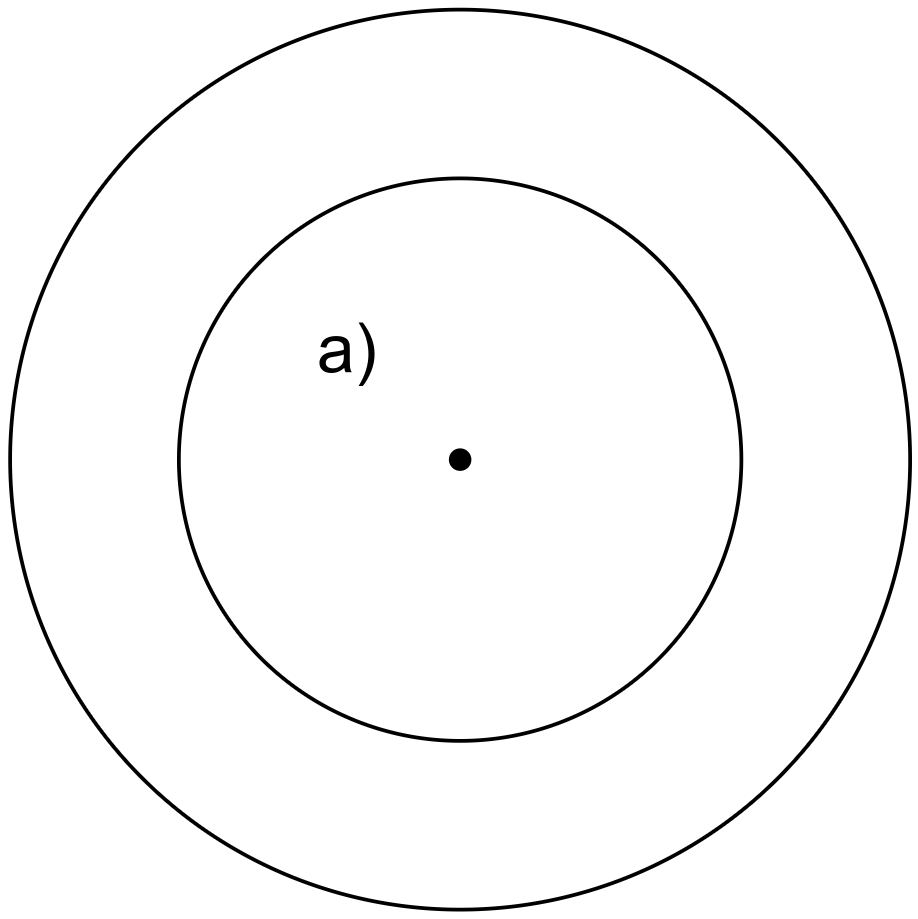
\includegraphics[height=0.35\textheight,keepaspectratio]{images/6/0_intersect.png}
    \end{center}
    \begin{center}
        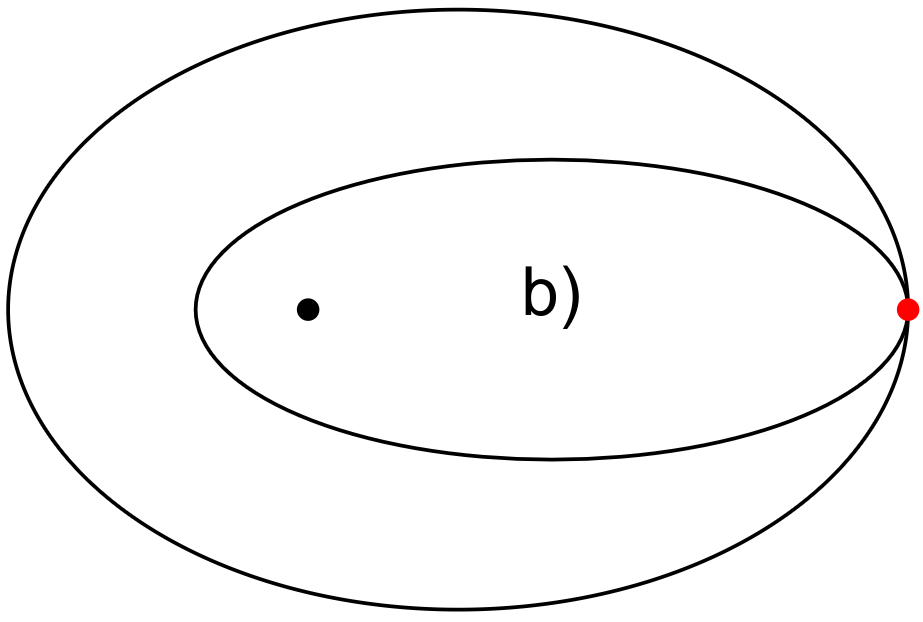
\includegraphics[height=0.25\textheight,keepaspectratio]{images/6/1_intersect.png}
    \end{center}
  \end{column}

  % правая колонка
  \begin{column}{0.49\textwidth}
    \begin{center}
        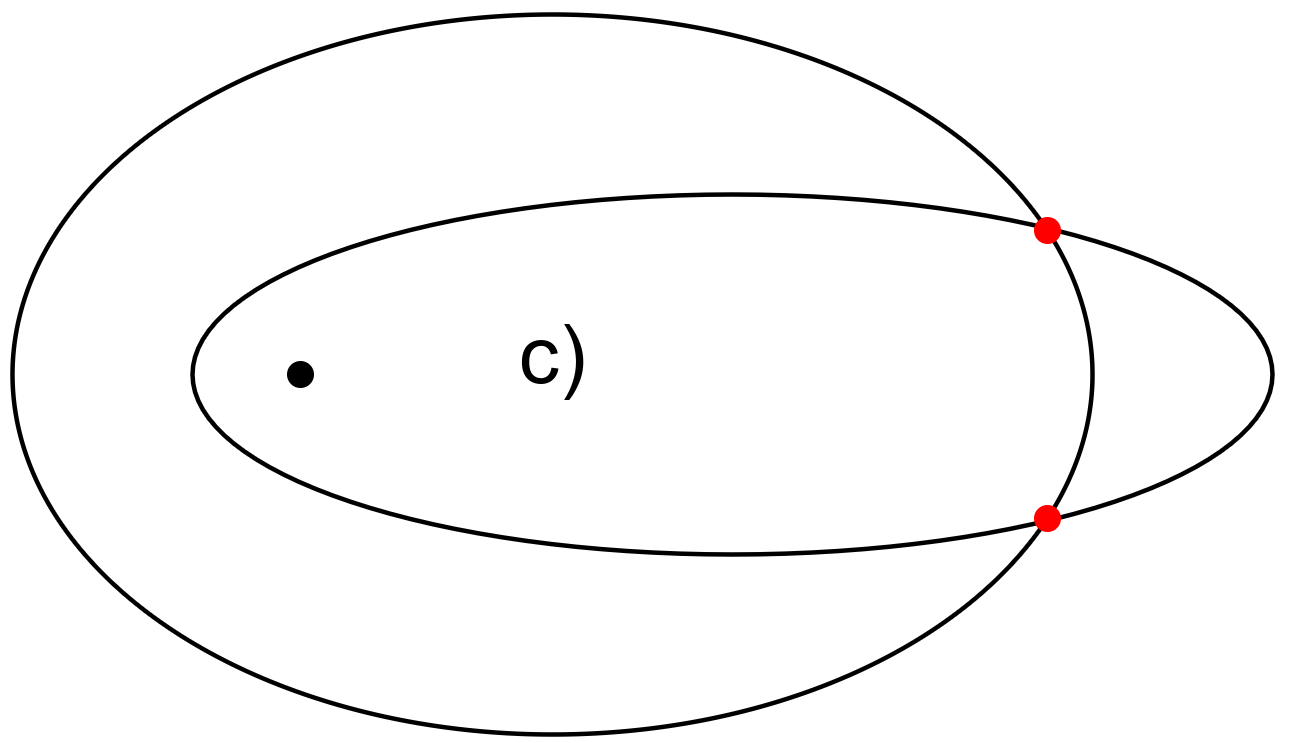
\includegraphics[height=0.25\textheight,keepaspectratio]{images/6/2_intersect.png}
    \end{center}
    \begin{center}
        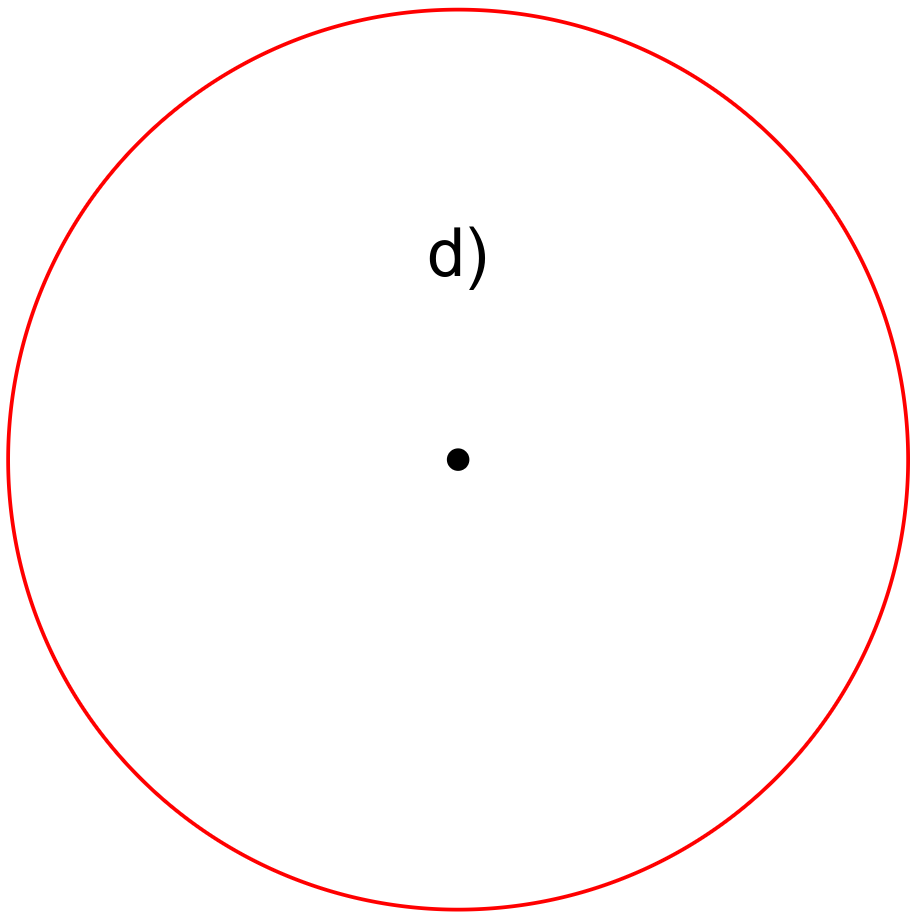
\includegraphics[height=0.35\textheight,keepaspectratio]{images/6/inf_intersect.png}
    \end{center}
  \end{column}
\end{columns}
\end{frame}

\begin{frame}{Компланарный одноимпульсный переход}
В плоскости каждая из орбит имеет 4 параметра: большую полуось $a$, эксцентриситет $e$, аргумент перицентра $\omega$ , истинную аномалию $\nu$. Уравнения для радиус-векторов каждой из орбит могут быть записаны так:
\begin{align*}
    \textbf{r}_1 &= \frac{p_1}{1 + e_1 \cos \nu_1} \left[ \cos (\nu_1 + \omega_1) \textbf{i} + \sin (\nu_1 + \omega_1) \textbf{j} \right], \\
    \textbf{r}_2 &= \frac{p_2}{1 + e_2 \cos \nu_2} \left[ \cos (\nu_2 + \omega_2) \textbf{i} + \sin (\nu_2 + \omega_2) \textbf{j} \right].
\end{align*}
В общей точке выполняется условие $\textbf{r}_1 = \textbf{r}_2$. Следовательно, будет справедливым:
\begin{gather*}
    \nu_1 + \omega_1 = \nu_2 + \omega_2, \\
    \frac{p_1}{1 + e_1 \cos \nu_1} = \frac{p_2}{1 + e_2 \cos \nu_2}.
\end{gather*}
Сделав несколько упрощений, мы можем получить:
\begin{equation*}
    (e_2 p_1 \cos \Delta \omega - e_1 p_2) \cos \nu_1 + (e_2 p_1 \sin \Delta \omega) \sin \nu_1 + (p_1 - p_2) = 0,
\end{equation*}
где $\Delta \omega = \omega_2 - \omega_1$, $\nu_2 = \nu_1 - \Delta \omega$. Это уравнение может иметь ноль, одно или два решения.
\end{frame}

\begin{frame}{Компланарный одноимпульсный переход}
\begin{columns}[T,totalwidth=\textwidth]
  % Левая колонка — постановка
  \begin{column}{0.48\textwidth}
    \begin{block}{Дано}
      \textbf{Начальная орбита}
      \begin{equation*}
          \begin{aligned}
            &a_1 = 10000~\text{км},\\
            &e_1 = 0.10,\\
            &\omega_1 = 20^{\circ}
          \end{aligned}
      \end{equation*}
      \medskip
      \textbf{Целевая орбита}
      \begin{equation*}
          \begin{aligned}
            &a_2 = 12000~\text{км},\\
            &e_2 = 0.35,\\
            &\omega_2 = 90^{\circ}
          \end{aligned}
      \end{equation*}
    \end{block}

    \begin{alertblock}{Найти}
      \begin{enumerate}[1)]
        \item Точки пересечения орбит;
        \item Импульс скорости $\Delta V$ в каждой точке.
      \end{enumerate}
    \end{alertblock}
  \end{column}

  % Правая колонка — место под рисунок/формулы
  \begin{column}{0.48\textwidth}
    \begin{exampleblock}{Решение}
        Решив уравнение относительно $\nu_1$, мы можем найти истинные аномалии точек пересечения орбит:
        \begin{center}
            \begin{tabular}{c c c}
                \toprule
                \textbf{Решение} & $\boldsymbol{\nu_1, ^\circ}$ & $\boldsymbol{\nu_2, ^\circ}$ \\
                \midrule
                1 & 8.8238   & -61.1762 \\
                2 & 166.5297 & 96.5297  \\
                \bottomrule
            \end{tabular}
        \end{center}
        В данном случае мы имеем две точки пересечения. Для решения 1 мы получаем следующие элементы:
        \begin{equation*}
            \begin{array}{r@{\;}c@{\;}l @{\qquad} r@{\;}c@{\;}l}
            a_1     & = & 10000~\text{км} & \Omega_1 & = & 0^\circ \\
            e_1     & = & 0.1                       & \omega_1 & = & 20^\circ \\
            i_1     & = & 0^\circ                   & \nu_1    & = & 8.8238^\circ
            \end{array}
        \end{equation*}
    \end{exampleblock}
  \end{column}
\end{columns}
\end{frame}

\begin{frame}{Компланарный одноимпульсный переход}
\begin{exampleblock}{Решение}
\begin{columns}[T,totalwidth=\textwidth]
  % Левая колонка — постановка
  \begin{column}{0.48\textwidth}
    Переведём их в декартовы элементы:
    \begin{align*}
        &\textbf{r}_1 = [7893.4512, \; 4343.7322, \; 0.0]~\text{км} \\
        &\textbf{v}_1 = [-3276.1964, \; 6155.4093, \; 0.0]~\text{м/с}
    \end{align*}
    Элементы целевой орбиты:
    \begin{equation*}
        \begin{array}{r@{\;}c@{\;}l @{\qquad} r@{\;}c@{\;}l}
        a_2     & = & 12000~\text{км} & \Omega_2 & = & 0^\circ \\
        e_2     & = & 0.35                      & \omega_2 & = & 90^\circ \\
        i_2     & = & 0^\circ                   & \nu_2    & = & -61.1762^\circ
        \end{array}
    \end{equation*}
    Соответствующие декартовы элементы:
    \begin{align*}
        &\textbf{r}_2 = [7893.4512, \; 4343.7322, \; 0.0]~\text{км} \\
        &\textbf{v}_2 = [-5119.6399, \; 5390.2834, \; 0.0]~\text{м/с}
    \end{align*}
  \end{column}

  % Правая колонка — место под рисунок/формулы
  \begin{column}{0.48\textwidth}
    Импульс, необходимый для перехода:
    \begin{align*}
        \Delta \textbf{v} &= \textbf{v}_2 - \textbf{v}_1 = \\
        &= [-1843.4434, \; -0765.1259, \; 0.0]~\text{м/с}
    \end{align*}
    \begin{equation*}
        \vert \vert \Delta \textbf{v} \vert \vert_2 = 1995.921~\text{м/с}
    \end{equation*}
    Аналогично, для второй точки, тот же метод даёт следующий результат:
    \begin{align*}
        \Delta \textbf{v} &= \textbf{v}_2 - \textbf{v}_1 = \\
        &= [-1958.2871, \; -404.7686, \; 0.0]~\text{м/с}
    \end{align*}
    \begin{equation*}
        \vert \vert \Delta \textbf{v} \vert \vert_2 = 1999.6815~\text{м/с}
    \end{equation*}
    Импульсы в обоих точках практически не различаются. Но решение 2 требует примерно на $4$ м/с меньше хар. скорости. 
  \end{column}
\end{columns}
\end{exampleblock}
\end{frame}

\begin{frame}{Некомпланарный одноимпульсный переход}
Важно заметить, что две некомпланарные орбиты могут иметь общие точки \textbf{только на линии пересечения плоскостей орбит}. 
\begin{columns}[T,totalwidth=\textwidth]
  % Левая колонка — постановка
  \begin{column}{0.48\textwidth}
    Направляющий вектор такой прямой может быть найден так:
    \begin{equation*}
        \mathbf{l} = \mathbf{h}_1 \times \mathbf{h}_2,
    \end{equation*}
    где $\mathbf{h} = \mathbf{r} \times \mathbf{v}$ - кинетический момент. Вектор $\mathbf{h}$ имеет явное выражение в кеплеровых элементах: 
    \begin{equation*}
        \mathbf{h} = [\sin i \sin \Omega, \; -\sin i \cos \Omega, \; \cos i].
    \end{equation*}
    Вектор перицентра орбиты:
    \begin{equation*}
    \mathbf{P} = 
    \begin{bmatrix}
        \cos \Omega \cos \omega - \sin \Omega \sin \omega \cos i \\
        \sin \Omega \cos \omega + \cos \Omega \sin \omega \cos i \\
        \sin \omega \sin i
    \end{bmatrix}
    \end{equation*}
  \end{column}

  % Правая колонка — место под рисунок/формулы
  \begin{column}{0.48\textwidth}
  Используя $\mathbf{h}$ и $\mathbf{P}$ мы можем найти значение $\nu$, соответствующее прямой пересечения плоскостей. Тогда мы сможем найти радиус вектора в этой точке для каждой из орбит и сравнить их:
  \begin{equation*}
      r = \frac{p}{1 + e \cos \nu}.
  \end{equation*}
    \begin{center}
        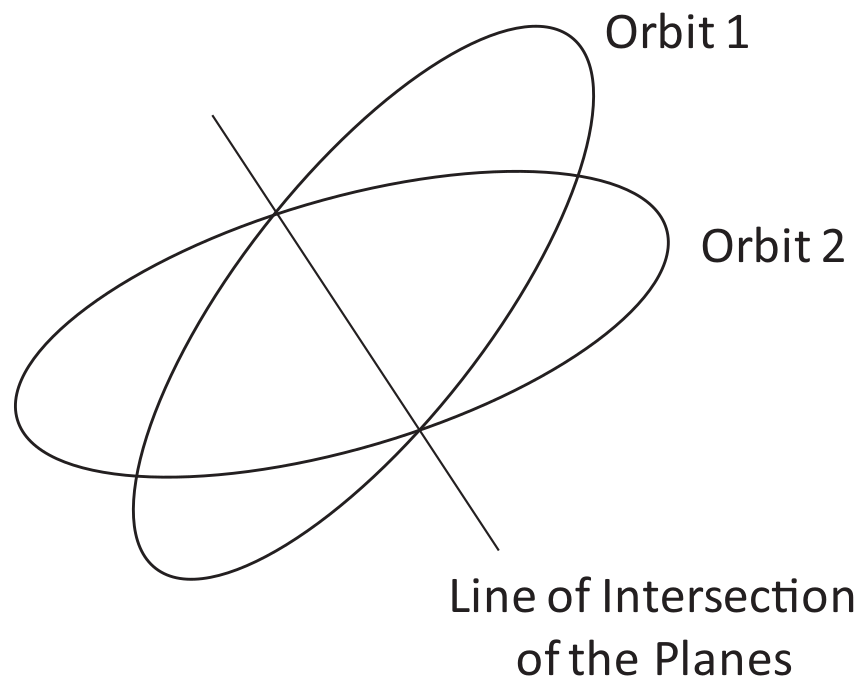
\includegraphics[height=0.4\textheight,keepaspectratio]{images/6/orb_intersection.png}
    \end{center}
  \end{column}
\end{columns}
\end{frame}

\begin{frame}{Некомпланарный одноимпульсный переход}
\begin{columns}[T,totalwidth=\textwidth]
  % Левая колонка — постановка
  \begin{column}{0.48\textwidth}
    \begin{block}{Дано}
      \textbf{Начальная орбита}
      \begin{equation*}
          \begin{array}{r@{\;}c@{\;}l @{\qquad} r@{\;}c@{\;}l}
            a_1 & = & 18654.3640~\text{км} & \Omega_1 & = & 89.44357^\circ \\
            e_1 & = & 0.28969592           & \omega_1 & = & 265.55428^\circ \\
            i_1 & = & 35.62718^\circ      
          \end{array}
      \end{equation*}
      \medskip
      \textbf{Целевая орбита}
      \begin{equation*}
          \begin{array}{r@{\;}c@{\;}l @{\qquad} r@{\;}c@{\;}l}
            a_2 & = & 20679.0085~\text{км} & \Omega_2 & = & 107.25881^\circ \\
            e_2 & = & 0.16932267           & \omega_2 & = & 234.60634^\circ \\
            i_2 & = & 38.46693^\circ      
          \end{array}
      \end{equation*}
    \end{block}

    \begin{alertblock}{Найти}
      \begin{enumerate}[1)]
        \item Точки пересечения орбит;
        \item Импульс скорости $\Delta V$ в каждой точке.
      \end{enumerate}
    \end{alertblock}
  \end{column}

  % Правая колонка — место под рисунок/формулы
  \begin{column}{0.48\textwidth}
    \begin{exampleblock}{Решение}
        Единичные нормали орбит:
        \begin{align*}
            &\mathbf{h}_1 = [0.582481, \; 0.005657, \; 0.812825], \\
            &\mathbf{h}_2 = [0.594054, \; 0.184559, \; 0.782967].
        \end{align*}
        Вектор прямой пересечения орбит (единичный):
        \begin{equation*}
            \mathbf{l} = [-0.804421, \; 0.139578, \; 0.577430].
        \end{equation*}
        Вектора перицентра:
        \begin{align*}
            &\mathbf{P}_1 = [0.809588, \; -0.085381, \; -0.580756], \\
            &\mathbf{P}_2 = [0.781369, \; -0.363746, \; -0.507101].
        \end{align*}
    \end{exampleblock}
  \end{column}
\end{columns}
\end{frame}

\begin{frame}{Некомпланарный одноимпульсный переход}
\begin{exampleblock}{Решение}
\begin{columns}[T,totalwidth=\textwidth]
  % Левая колонка — постановка
  \begin{column}{0.45\textwidth}
    Истинные аномалии, связанные с $+\mathbf{l}$:
    \begin{align*}
        &\nu_1 = 176.87444^\circ, \\
        &\nu_2 = 193.55737^\circ
    \end{align*}
    и соответствующие им радиусы:
    \begin{align*}
        &r_1 = 24\;043.8698~\text{км}, \\
        &r_2 = 24\;043.8698~\text{км}
    \end{align*}
    Получаем точку пересечения.
    Для противоположной точки орбиты ($-\mathbf{l}$):
    \begin{align*}
        &\nu_1 = 356.87444^\circ, \\
        &\nu_2 = 13.55737^\circ
    \end{align*}
    Соответствующие им радиусы:
    \begin{align*}
        &r_1 = 13\;254.6997~\text{км}, \\
        &r_2 = 17\;247.1734~\text{км}
    \end{align*}
  \end{column}

  % Правая колонка — место под рисунок/формулы
  \begin{column}{0.50\textwidth}
    Это не точка пересечения. Вернёмся к найденной точке пересечения и найдём декартовы элементы начальной и целевой орбит:
    \begin{align*}
        &\textbf{r}_1 = [-19\;341.3822, \; 3\;355.9985, \; 13\;883.6552]~\text{км} \\
        &\textbf{v}_1 = [-462.0134, \; -3\;388.2745, \; 307.5039]~\text{м/с}
    \end{align*}
    \begin{align*}
        &\textbf{r}_2 = [-19\;341.3822, \; 3\;355.9985, \; 13\;883.6552]~\text{км} \\
        &\textbf{v}_2 = [132.1320, \; -3\;645.1333, \; 758.9694]~\text{м/с}
    \end{align*}
    Требуемый импульс:
    \begin{align*}
        \Delta \textbf{v} &= \textbf{v}_2 - \textbf{v}_1 = \\
        &= [594.1453, \; -256.8588, \; 451.4655]~\text{м/с}
    \end{align*}
    \begin{equation*}
        \vert \vert \Delta \textbf{v} \vert \vert_2 = 789.1807~\text{м/с}
    \end{equation*}
  \end{column}
\end{columns}
\end{exampleblock}
\end{frame}

\begin{frame}{Коррекция ограниченного набора орбитальных элементов}
Вместо того, чтобы пытаться скорректировать весь набор орбитальных элементов $(a, e, \omega, i, \Omega)$, мы попытаемся скорректировать уменьшенный набор элементов. Мотивацией к этому может служить следующее:
\begin{itemize}
    \item Скорректировать полный набор орбитальных элементов удаётся лишь в специфических случаев (орбиты имеют общую точку);
    \item Часто, для успешного функционирования, КА должен сохранять некоторые (или всё) свои орбитальные элементы внутри заданного диапазона (\textbf{orbit box});
    \item Часто, внешние возмущения сильнее изменяют некоторые элементы орбиты, в отличие о других.
\end{itemize}
Вследствие чего, возникает необходимость корректировать ограниченный набор орбитальных элементов. 
\end{frame}

\begin{frame}{Коррекция элементов в плоскости}
Манёвр в плоскости задаётся двумя компонентами: $\Delta V = [\Delta V_r, \; \Delta V_t, \; 0]$. Таким образом, имея две свободных переменных, мы можем рассчитывать удовлетворить двум ограничениям, например, $a$ и $e$, $a$ и $\omega$, $r_p$ и $\nu$. Важно заметить, что остальные орбитальные элементы могут меняться, возможно значительно. 

Перед тем как рассматривать конкретные задачи, отметим несколько общих вещей. Импульсный манёвр в плоскости не изменяет аргумент широты ($u = u_1 = u_2$). Это даёт нам информацию об орбите после импульса.

Вектор восходящего узла орбиты задаётся следующим выражением:
\begin{equation*}
    \boldsymbol{\Omega} = [\cos \Omega, \; \sin \Omega, \; 0].
\end{equation*}
Единичный вектор, нормальный к орбите:
\begin{equation*}
    \mathbf{h} = \frac{\mathbf{r} \times \mathbf{v}}{\vert \mathbf{r} \times \mathbf{v} \vert} = [\sin i \sin \Omega, \; -\sin i \cos \Omega, \; \cos i].
\end{equation*}
Аргумент широты может быть найден как знаковый угол от $\boldsymbol{\Omega}$ до вектора $\mathbf{r}$, с положительным направлением против часовой стрелки, если смотреть на вектор $\mathbf{h}$. Таким образом мы уже знаем три постманевровых параметра: $u_2, \; i_2, \; \Omega_2$.
\end{frame}

\begin{frame}{Коррекция $a$, $e$}
Если задана целевая большая полуось $a_2$ и эксцентриситет $e_2$, то истинная аномалия на целевой орбите может быть рассчитана из уравнения конического сечения:
\begin{equation*}
    r = \frac{a_2 (1 - e_2^2)}{1 + e_2 \cos \nu_2} \quad \longrightarrow \quad 
    \cos \nu_2 = \frac{1}{e_2} \left[ \frac{a_2}{r} (1 - e_2^2) - 1 \right].
\end{equation*}
Это уравнения имеет два решения: положительное $\nu_{2a}$ и отрицательное $\nu_{2b}$. Тогда аргумент перицентра может быть найден так:
\begin{equation*}
    w_{2a} = u - \nu_{2a}, \quad \quad w_{2b} = u - \nu_{2b},
\end{equation*}
Теперь мы знаем весь набор целевых кеплеровых элементов. Переведём их в декартовы элементы и найдём требуемые импульсы скорости.
\begin{equation*}
    \Delta \mathbf{v}_a = \mathbf{v}_{2a} - \mathbf{v}_1, \quad \quad
    \Delta \mathbf{v}_b = \mathbf{v}_{2b} - \mathbf{v}_1.
\end{equation*}
Следующие комбинации элементов могут быть получены, используя описанный алгоритм, с помощью конвертации их в большую полуось и эксцентриситет:
\begin{equation*}
 a, \; r_p \quad \quad a, \; r_a \quad \quad a, \; p \quad \quad
 e, \; r_p \quad \quad e, \; r_a \quad \quad e, \; p \quad \quad
 r_p, \; r_a \quad \quad r_p, \; p \quad \quad r_a, \; p \quad \quad
\end{equation*}
Все эти комбинации также имеют два решения.
\end{frame}

\begin{frame}{Коррекция $a$, $e$}
\begin{columns}[T,totalwidth=\textwidth]
  % Левая колонка — постановка
  \begin{column}{0.48\textwidth}
    \begin{block}{Дано}
      \textbf{Начальная орбита}
      \begin{equation*}
          \begin{array}{r@{\;}c@{\;}l @{\qquad} r@{\;}c@{\;}l}
            a_1 & = & 26\;000~\text{км} & \Omega_1 & = & 0^\circ \\
            e_1 & = & 0.6               & \omega_1 & = & 250^\circ \\
            i_1 & = & 64^\circ          & \nu_1 & = & 60^\circ
          \end{array}
      \end{equation*}
      \medskip
      \textbf{Целевые элементы}
      \begin{align*}
            &a_2 = 26\;554~\text{км} \\
            &e_2 = 0.7   
      \end{align*}
    \end{block}

    \begin{alertblock}{Найти}
      \begin{enumerate}[1)]
        \item Импульс скорости $\Delta V$, необходимый для осуществления коррекции.
      \end{enumerate}
    \end{alertblock}
  \end{column}

  % Правая колонка — место под рисунок/формулы
  \begin{column}{0.48\textwidth}
    \begin{exampleblock}{Решение}
    Используя описанный алгоритм, мы получаем следующие орбиты, имеющие целевые большую полуось и эксцентриситет:  
        \begin{center}
            \begin{tabular}{c c c}
                \toprule
                \textbf{Э} & $a$ & $b$ \\
                \midrule
                $a$, км          & 26\;554 & 26\;554 \\
                $e$              & 0.7     & 0.7  \\
                $\omega, ^\circ$ & 224.754 & 35.246 \\
                $i, ^\circ$      & 64      & 64 \\
                $\Omega, ^\circ$ & 0       & 0 \\
                $\nu, ^\circ$    & 85.246  & 274.754 \\
                \bottomrule
            \end{tabular}
        \end{center}
    \end{exampleblock}
  \end{column}
\end{columns}
\end{frame}

\begin{frame}{Коррекция $a$, $e$}
\begin{columns}[T,totalwidth=\textwidth]
  % Левая колонка — постановка
  \begin{column}{0.53\textwidth}
    \begin{exampleblock}{Решение}
        Получим декартовы элементы:
        \begin{align*}
            &\textbf{r}_1 = [8\;227.6814, \; -4\;298.3908, \; -8813.0072]~\text{км} \\
            &\textbf{v}_1 = [6\;508.7585, \; 938.8305, \; 1\;924.8879]~\text{м/с}
        \end{align*}
        \begin{align*}
            &\textbf{r}_a = [8\;227.6814, \; -4\;298.3908, \; -8813.0072]~\text{км} \\
            &\textbf{v}_a = [6\;829.7618, \; 346.4893, \; 710.4084]~\text{м/с}
        \end{align*}
        \begin{align*}
            &\textbf{r}_b = [8\;227.6814, \; -4\;298.3908, \; -8813.0072]~\text{км} \\
            &\textbf{v}_b = [1\;964.3695, \; 2\;888.3181, \; 5\;921.9298]~\text{м/с}
        \end{align*}
        \begin{align*}
            \Delta \textbf{v}_1 &= \textbf{v}_a - \textbf{v}_1 = \\
            &= [321.0033, \; -592.3412, \; -1\;214.4795]~\text{м/с}
        \end{align*}
        \begin{equation*}
            \vert \vert \Delta \textbf{v}_1 \vert \vert_2 = 1\;388.8382~\text{м/с}
        \end{equation*}
    \end{exampleblock}
  \end{column}

  % Правая колонка — место под рисунок/формулы
  \begin{column}{0.45\textwidth}
    \begin{exampleblock}{Решение}
        \begin{align*}
            &\Delta \textbf{v}_2 = \textbf{v}_b - \textbf{v}_1 = \\
            &=[-4\;544.3889, \; 1\;949.4876, \; 3\;997.0419]~\text{м/с}
        \end{align*}
        \begin{equation*}
            \vert \vert \Delta \textbf{v}_2 \vert \vert_2 = 6\;358.3266~\text{м/с}
        \end{equation*}
    \end{exampleblock}
    \begin{center}
        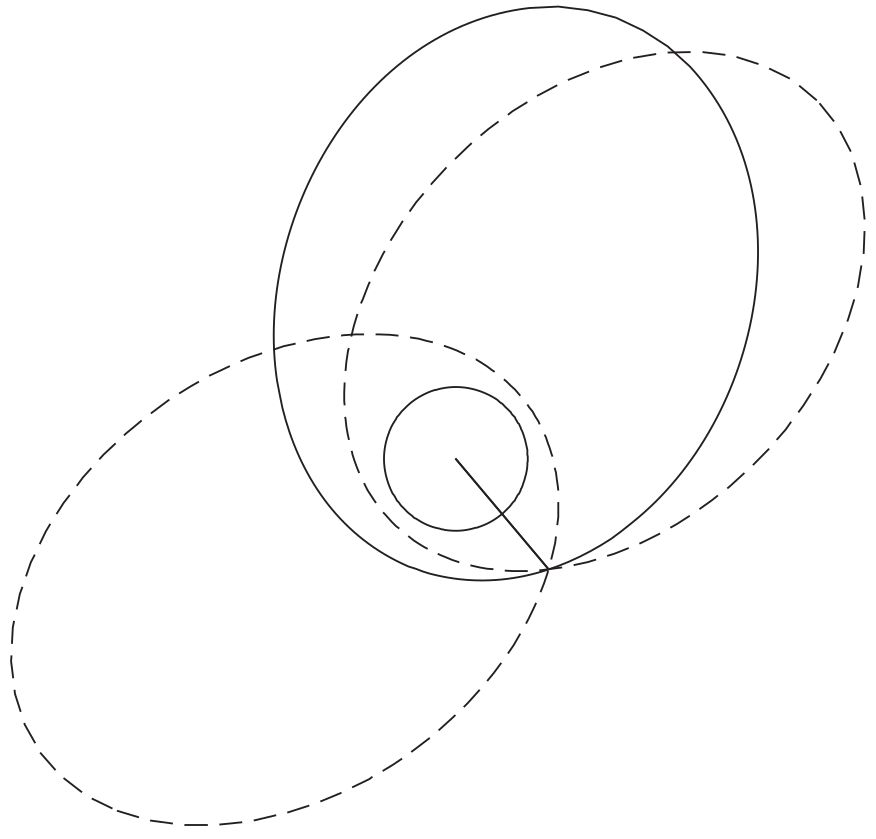
\includegraphics[height=0.50\textheight,keepaspectratio]{images/6/a_e_correction.png}
    \end{center}
  \end{column}
\end{columns}
\end{frame}

\begin{frame}{Оптимизация коррекции $a$, $e$}
\begin{center}
    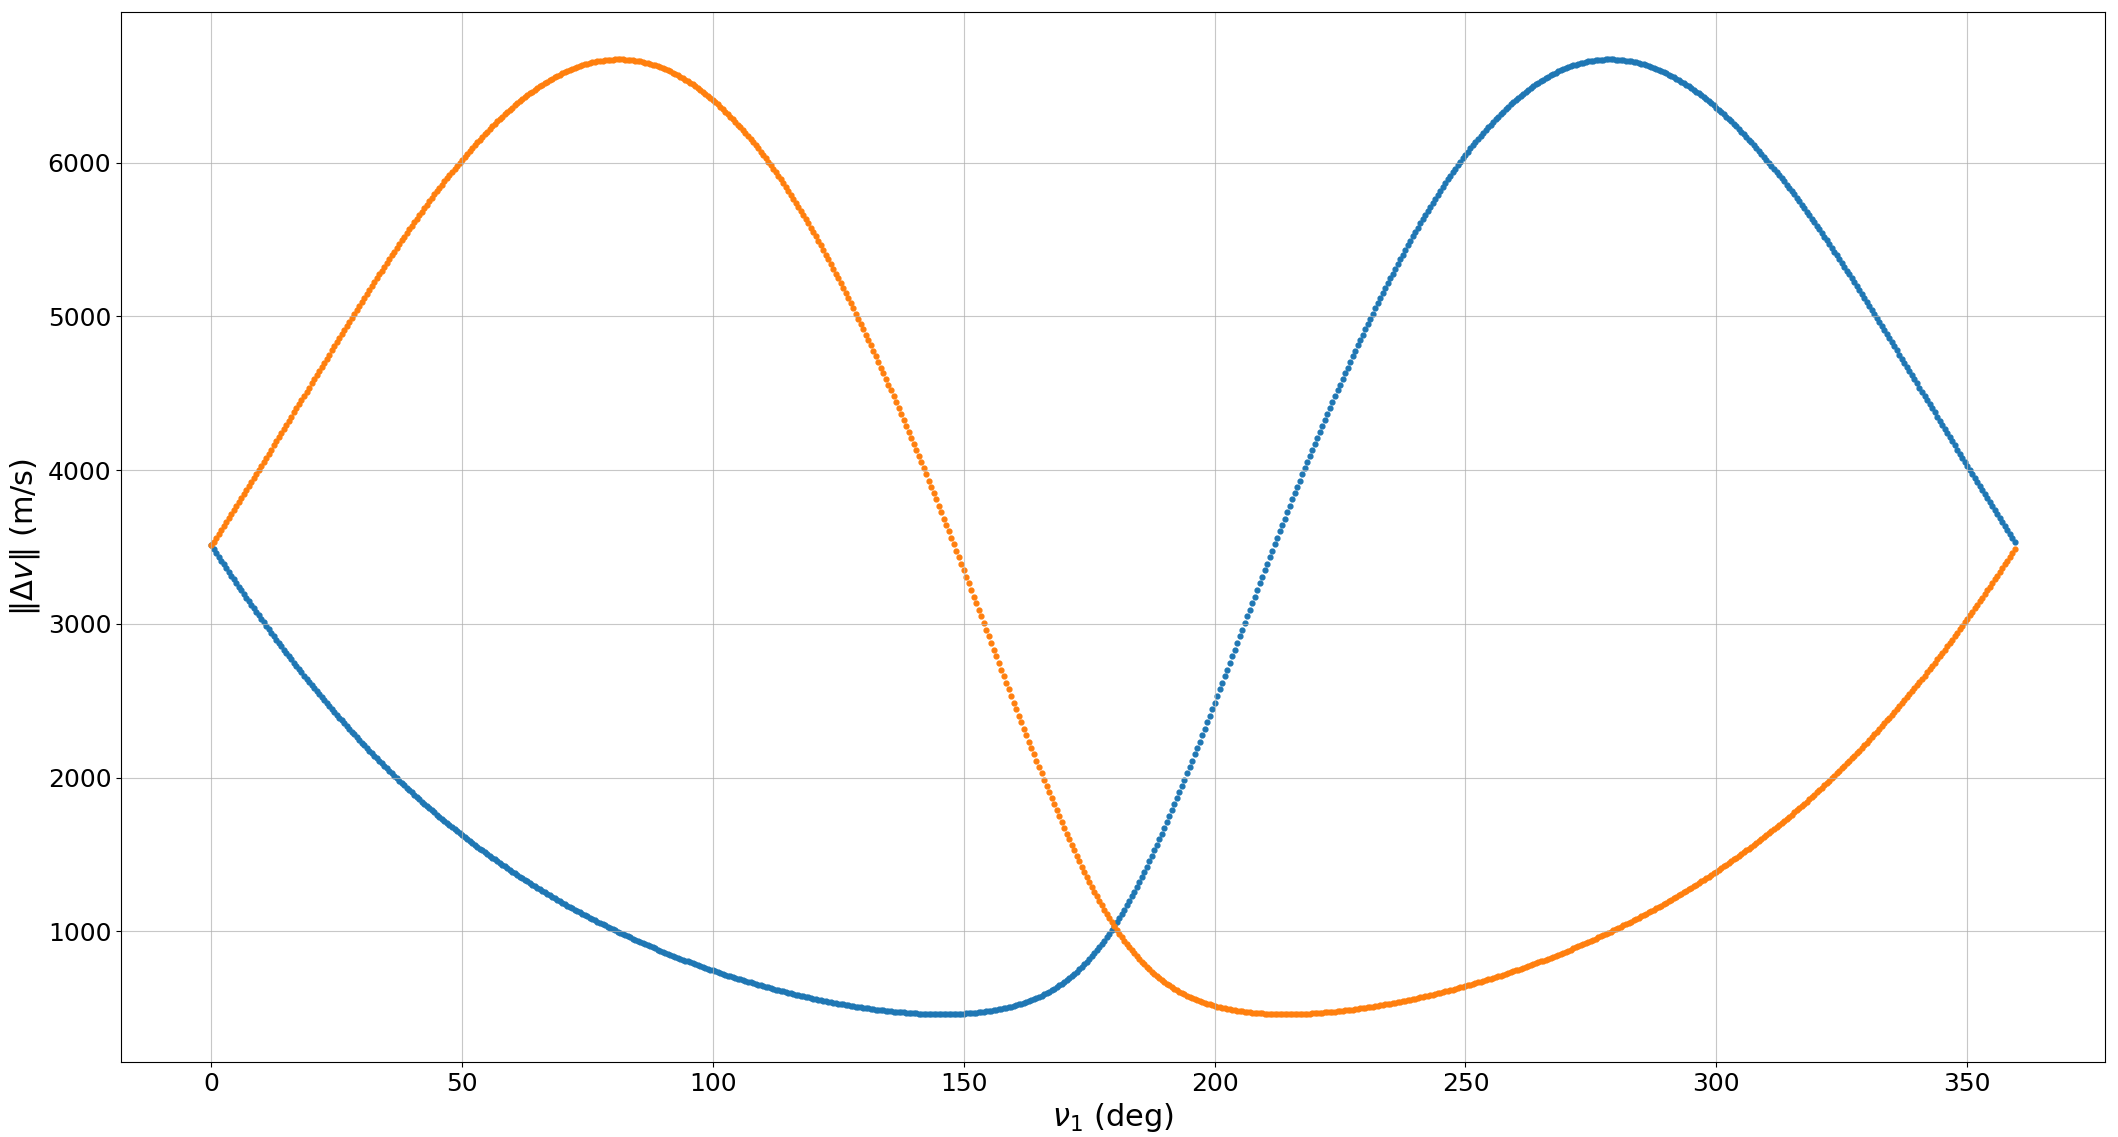
\includegraphics[height=0.70\textheight,keepaspectratio]{images/6/a_e_opt.png}
\end{center}
\end{frame}

\begin{frame}{Коррекция $a$, $\omega$}
Имея известный аргумент широты $u$ и аргумент перицентра целевой орбиты $\omega_2$, мы должны найти эксцентриситет и истинную аномалию целевой орбиты. Зная, что $u = u_1 = u_2$, мы можем рассчитать истинную аномалию:
\begin{equation*}
    \nu_2 = u - \omega_2.
\end{equation*}
Уравнение конического сечения может быть преобразовано так:
\begin{equation*}
    r = \frac{a_2 (1 - e_2^2)}{1 + e_2 \cos \nu_2} \quad \longrightarrow \quad 
    a_2 e_2^2 + (r \cos \nu_2) e_2 + r - a_2 = 0.
\end{equation*}
Это квадратное уравнение может давать до двух значений эксцентриситета целевой орбиты. Таким образом мы можем полностью определить постманевровые значения орбитальных элементов.
\end{frame}

\begin{frame}{Коррекция $a$, $\omega$}
\begin{columns}[T,totalwidth=\textwidth]
  % Левая колонка — постановка
  \begin{column}{0.48\textwidth}
    \begin{block}{Дано}
      \textbf{Начальная орбита}
      \begin{equation*}
          \begin{array}{r@{\;}c@{\;}l @{\qquad} r@{\;}c@{\;}l}
            a_1 & = & 26\;222~\text{км} & \Omega_1 & = & 0^\circ \\
            e_1 & = & 0.7               & \omega_1 & = & 266^\circ \\
            i_1 & = & 63.434^\circ      & \nu_1 & = & 222^\circ
          \end{array}
      \end{equation*}
      \medskip
      \textbf{Целевые элементы}
      \begin{align*}
            &a_2 = 26\;554~\text{км} \\
            &\omega_2 = 270^\circ  
      \end{align*}
    \end{block}

    \begin{alertblock}{Найти}
      \begin{enumerate}[1)]
        \item Импульс скорости $\Delta V$, необходимый для осуществления коррекции.
      \end{enumerate}
    \end{alertblock}
  \end{column}

  % Правая колонка — место под рисунок/формулы
  \begin{column}{0.48\textwidth}
    \begin{exampleblock}{Решение}
    Используя описанный алгоритм, мы получаем следующие орбиты, имеющие целевые большую полуось и аргумент перицентра:  
        \begin{center}
            \begin{tabular}{c c c}
                \toprule
                \textbf{Э} & $a$ & $b$ \\
                \midrule
                $a$, км          & 26\;554  & 26\;554 \\
                $e$              & 0.761972 & 0.0651679  \\
                $\omega, ^\circ$ & 270      & 270 \\
                $i, ^\circ$      & 63.434   & 63.434 \\
                $\Omega, ^\circ$ & 0        & 0 \\
                $\nu, ^\circ$    & 218      & 218 \\
                \bottomrule
            \end{tabular}
        \end{center}
    \end{exampleblock}
  \end{column}
\end{columns}
\end{frame}

\begin{frame}{Коррекция $a$, $\omega$}
\begin{columns}[T,totalwidth=\textwidth]
  % Левая колонка — постановка
  \begin{column}{0.55\textwidth}
    \begin{exampleblock}{Решение}
        Получим декартовы элементы:
        \begin{align*}
            &\textbf{r}_1 = [-17\;160.0667, \; 9\;822.8728, \;19\;644.9322]~\text{км} \\
            &\textbf{v}_1 = [-489.8018, \; -1\;622.4428, \; -3\;244.7512]~\text{м/с}
        \end{align*}
        \begin{align*}
            &\textbf{r}_a = [-17\;160.0667, \; 9\;822.8728, \;19\;644.9322]~\text{км} \\
            &\textbf{v}_a = [-155.7771, \; -1\;647.2598, \; -3\;294.3832]~\text{м/с}
        \end{align*}
        \begin{align*}
            &\textbf{r}_b = [-17\;160.0667, \; 9\;822.8728, \;19\;644.9322]~\text{км} \\
            &\textbf{v}_b = [-2\;806.5448, \; -1\;069.0535, \; -2\;138.0184]~\text{м/с}
        \end{align*}
        \begin{align*}
            \Delta \textbf{v}_1 &= \textbf{v}_a - \textbf{v}_1 = \\
            &= [334.0247, \; -24.8170, \; -49.6320]~\text{м/с}
        \end{align*}
        \begin{equation*}
            \vert \vert \Delta \textbf{v}_1 \vert \vert_2 = 338.6026~\text{м/с}
        \end{equation*}
    \end{exampleblock}
  \end{column}

  % Правая колонка — место под рисунок/формулы
  \begin{column}{0.50\textwidth}
    \begin{exampleblock}{Решение}
        \begin{align*}
            &\Delta \textbf{v}_2 = \textbf{v}_b - \textbf{v}_1 = \\
            &=[-2\;316.7429, \; 553.3893, \; 1\;106.7327]~\text{м/с}
        \end{align*}
        \begin{equation*}
            \vert \vert \Delta \textbf{v}_2 \vert \vert_2 = 2\;626.4796~\text{м/с}
        \end{equation*}
    \end{exampleblock}
    \begin{center}
        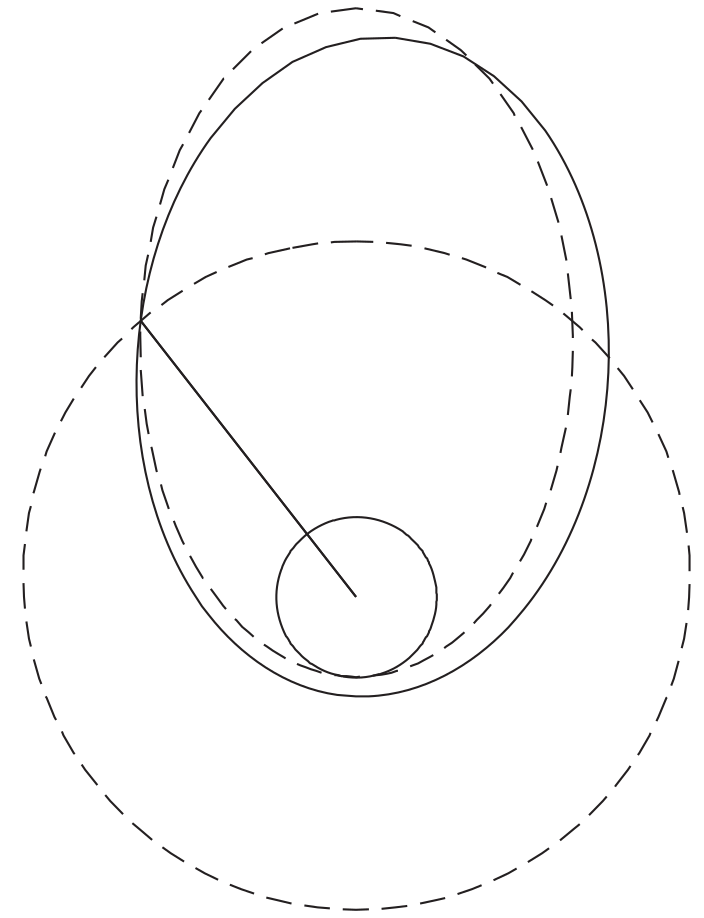
\includegraphics[height=0.50\textheight,keepaspectratio]{images/6/a_w_correction.png}
    \end{center}
  \end{column}
\end{columns}
\end{frame}

\begin{frame}{Оптимизация коррекции $a$, $\omega$}
\begin{center}
    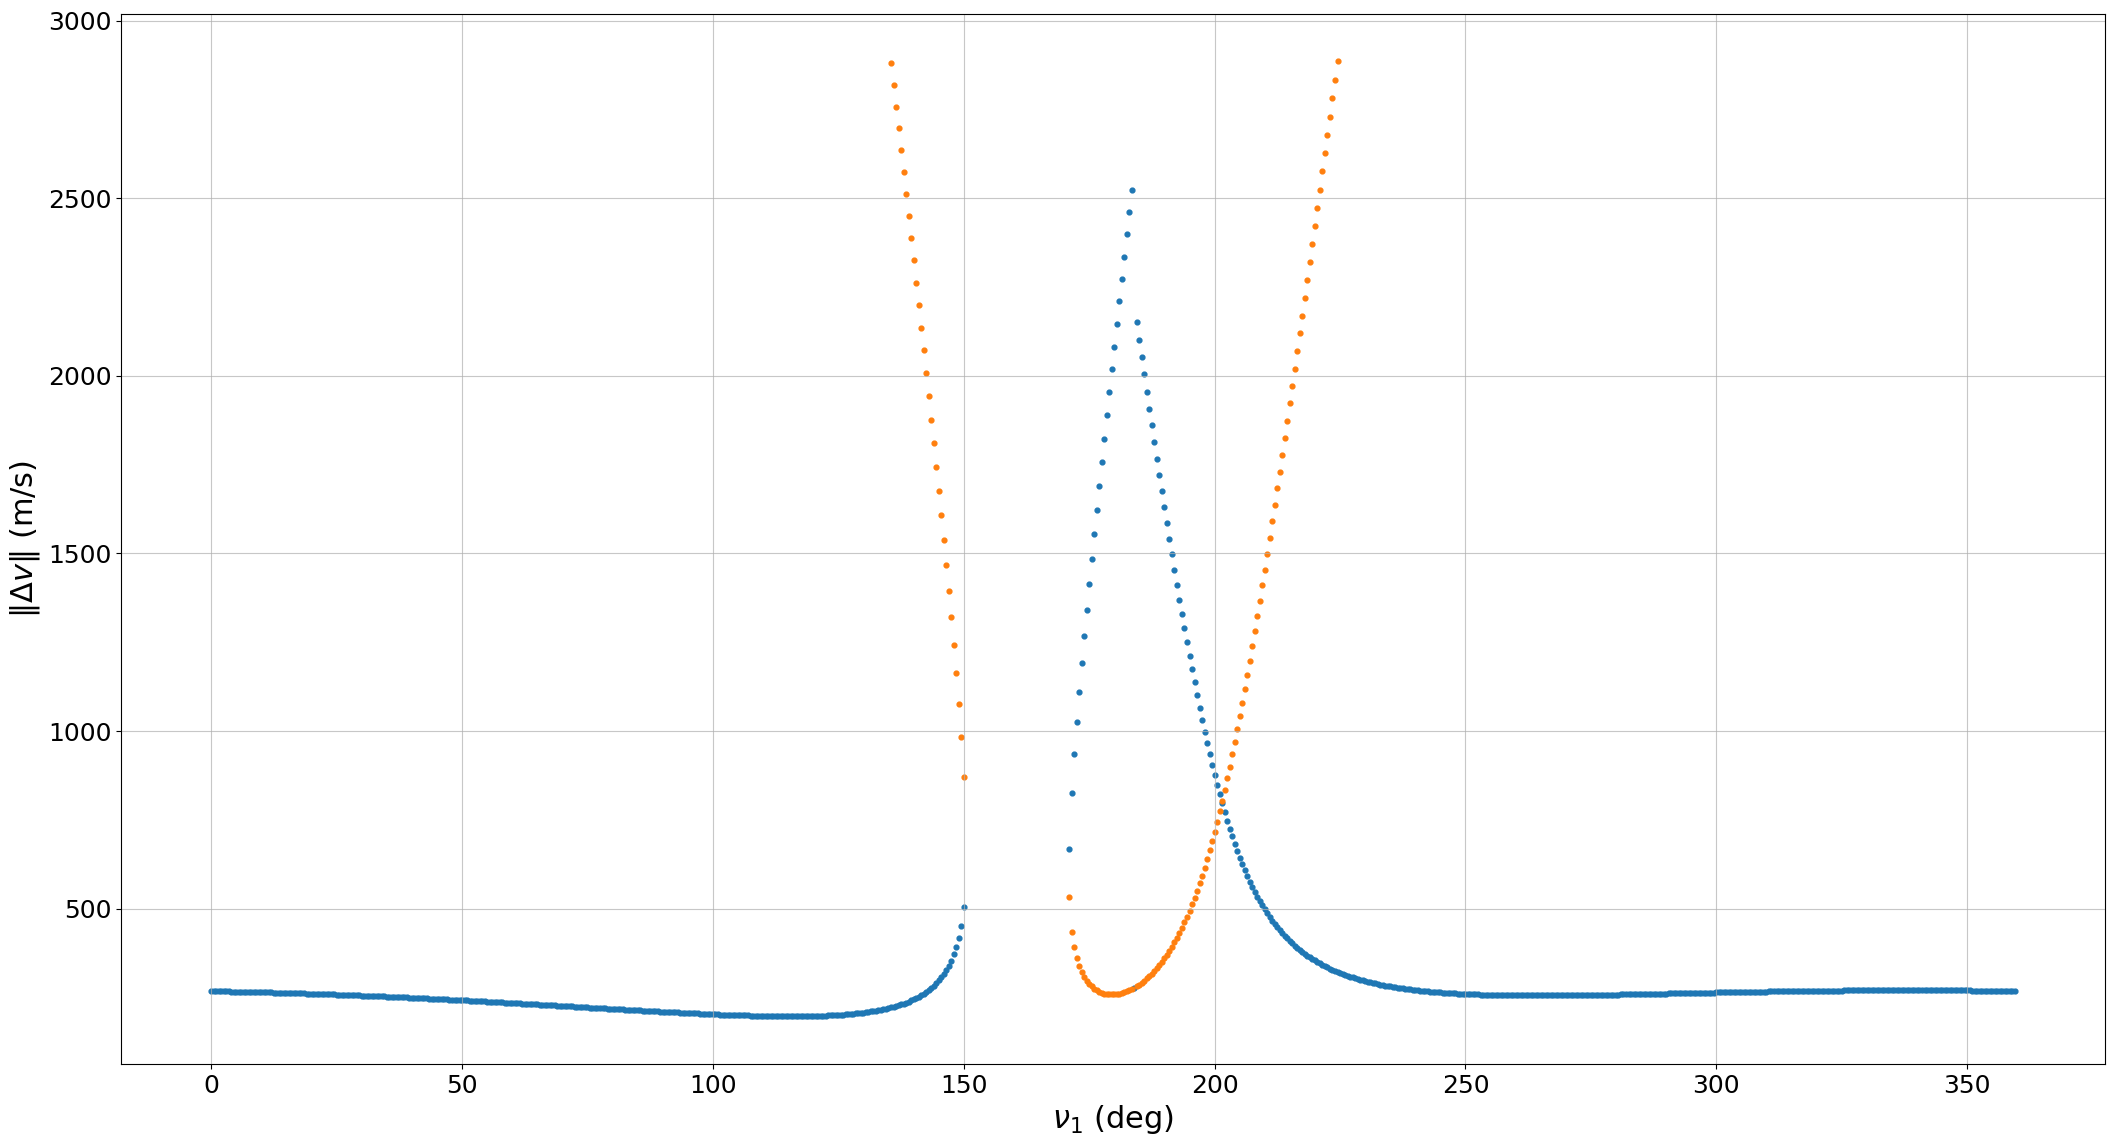
\includegraphics[height=0.70\textheight,keepaspectratio]{images/6/a_w_opt.png}
\end{center}
\end{frame}

\begin{frame}{Недопустимые случаи}
Существует множество комбинаций начальных и целевых орбитальных элементов, которые нельзя получить одним импульсом. Вот некоторые простые случаи:
\begin{itemize}
    \item $a/e$: В случае если целевые большая полуось и эксцентриситет такие, что результирующий радиус перицентра выше, чем радиус текущей точки.
    \item $r_p$: В случае, если целевой радиус перицентра больше, чем радиус текущей точки.
    \item $r_a$: В случае, если целевой радиус апоцентра меньше, чем радиус текущей точки.
\end{itemize}
\end{frame}

\begin{frame}{Коррекция элементов вне плоскости}
В общем случае точечный импульс имеет три степени свободы, а это значит, что мы можем попытаться удовлетворить ещё одному граничному условию. Мы сможем скорректировать два внутриплоскостных параметра и либо наклонение $i$, либо долготу восходящего узла $\Omega$. В общем случае $i$ и $\Omega$ не могут быть одновременно скомпенсированы.

Единичный вектор, нормальный к орбите:
\begin{equation*}
    \mathbf{h} = \frac{\mathbf{r} \times \mathbf{v}}{\vert \mathbf{r} \times \mathbf{v} \vert} = [\sin i \sin \Omega, \; -\sin i \cos \Omega, \; \cos i].
\end{equation*}
Рассмотрим скалярное произведение:
\begin{equation*}
    \langle \mathbf{r}, \mathbf{h} \rangle = r_x \sin i \sin \Omega - r_y \sin i \cos \Omega + r_z \cos i = 0.
\end{equation*}
Тогда если:
\begin{itemize}
    \item \textbf{Задана} $\Omega_2$. Решение сводится к следующему:
    \begin{equation*}
        \tan i_2 = \frac{-r_z}{r_x \sin \Omega_2 - r_y \cos \Omega_2},
    \end{equation*}
    что даёт единственное решение в диапазоне $[-\pi; \; \pi]$.

    \item \textbf{Задано} $i_2$. Уравнение выше может иметь ноль, одно и два решения. Если решений нет, значит задан невозможный переход. Пример: геоцентрическая широта с точке манёвра больше желаемого постманеврового наклонения.
\end{itemize}
\end{frame}

\begin{frame}{Коррекция $a$, $e$, $\Omega$}
\begin{columns}[T,totalwidth=\textwidth]
  % Левая колонка — постановка
  \begin{column}{0.48\textwidth}
    \begin{block}{Дано}
      \textbf{Начальная орбита}
      \begin{equation*}
          \begin{array}{r@{\;}c@{\;}l @{\qquad} r@{\;}c@{\;}l}
            a_1 & = & 26\;000~\text{км} & \Omega_1 & = & 0^\circ \\
            e_1 & = & 0.6               & \omega_1 & = & 250^\circ \\
            i_1 & = & 64^\circ          & \nu_1 & = & 60^\circ
          \end{array}
      \end{equation*}
      \medskip
      \textbf{Целевые элементы}
      \begin{align*}
            &a_2 = 26\;554~\text{км} \\
            &e_2 = 0.7               \\ 
            &\Omega_2 = 3^\circ
      \end{align*}
    \end{block}

    \begin{alertblock}{Найти}
      \begin{enumerate}[1)]
        \item Импульс скорости $\Delta V$, необходимый для осуществления коррекции.
      \end{enumerate}
    \end{alertblock}
  \end{column}

  % Правая колонка — место под рисунок/формулы
  \begin{column}{0.48\textwidth}
    \begin{exampleblock}{Решение}
        Используйте алгоритм для коррекции большой полуоси и эксцентриситета и выражение для нахождения целевого наклонения с предыдущего слайда.
    \end{exampleblock}
  \end{column}
\end{columns}
\end{frame}

\begin{frame}{Оптимизация коррекции $a$, $e$, $\Omega$}
\begin{center}
    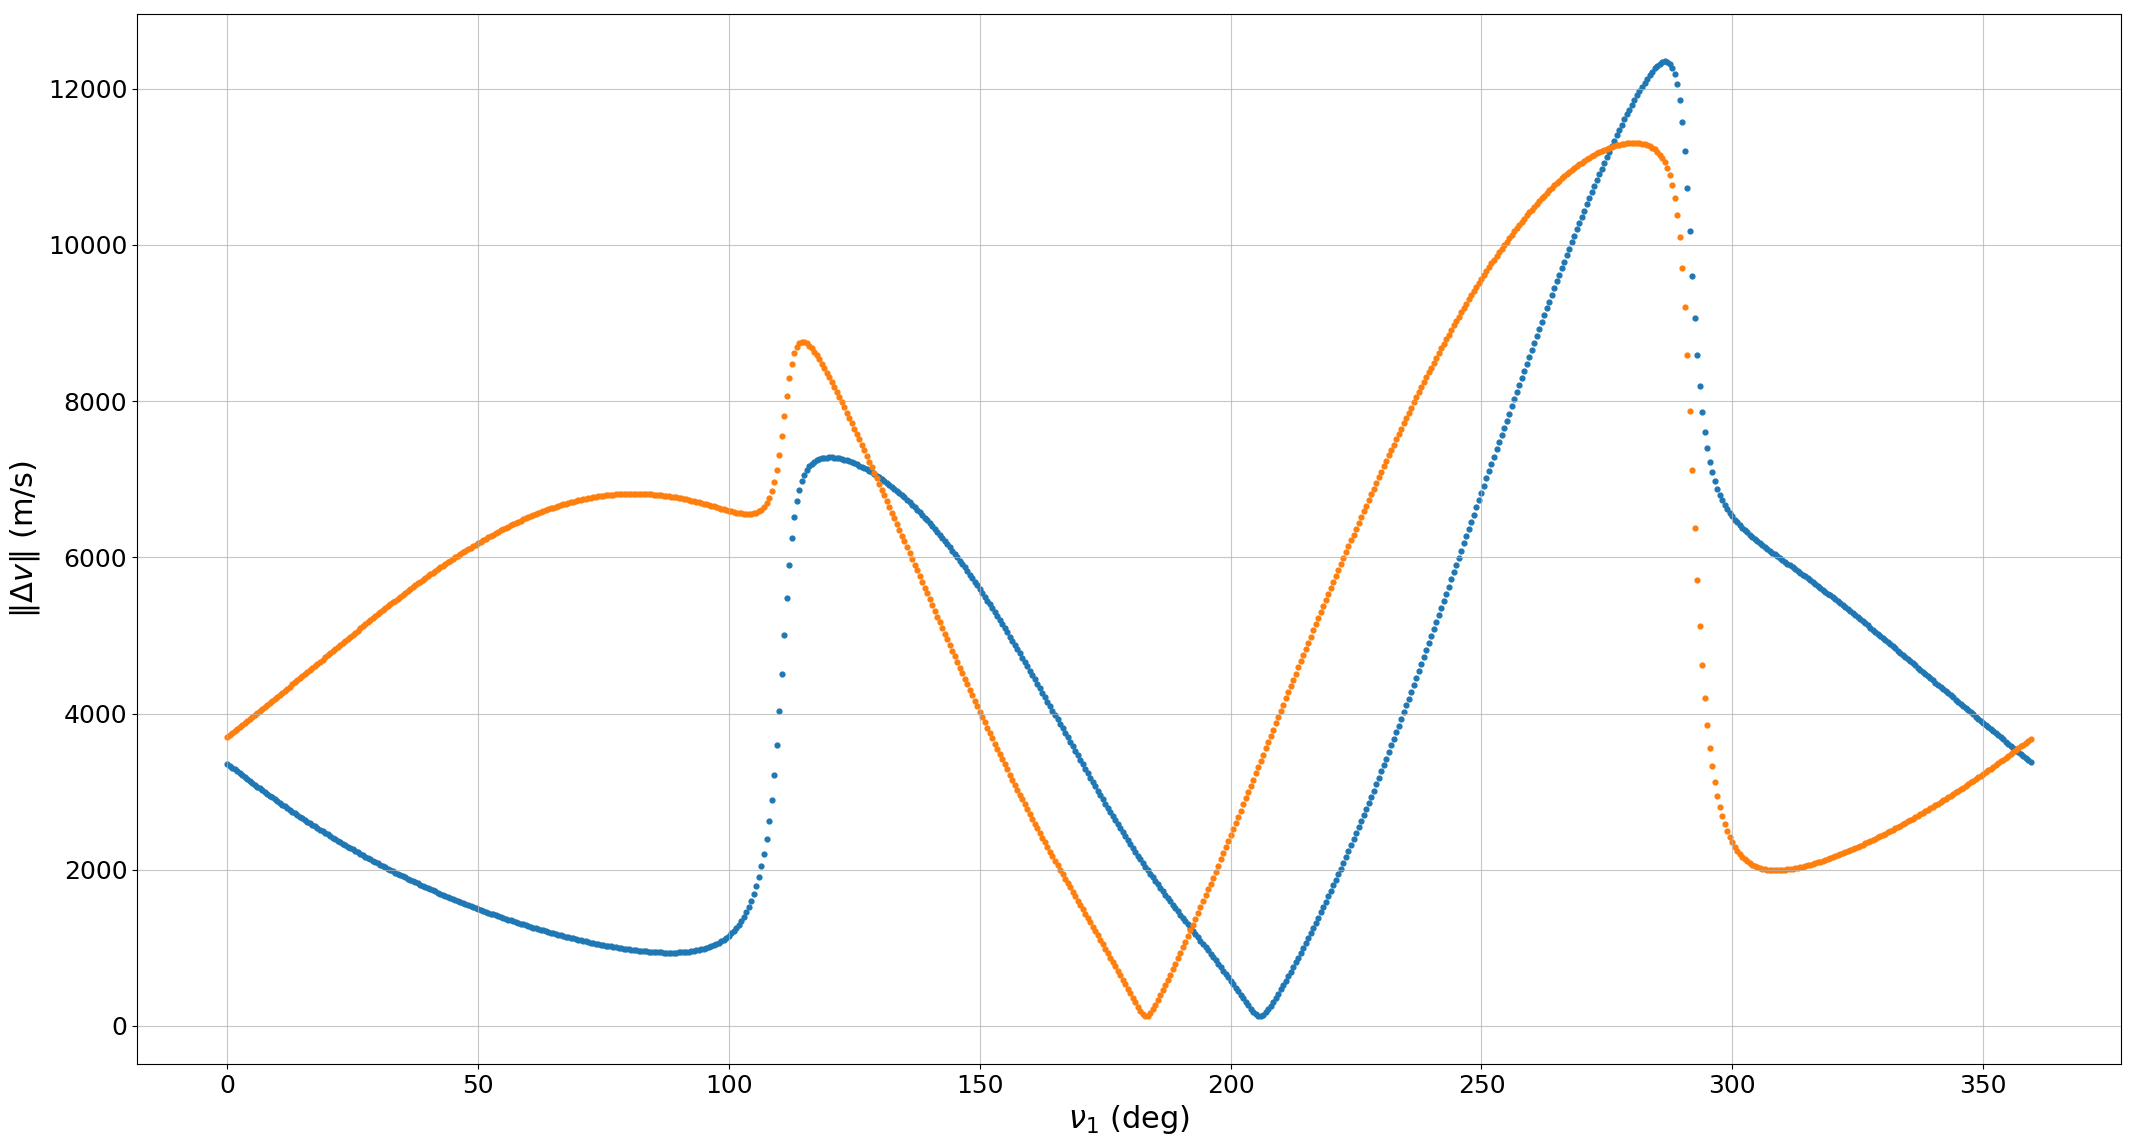
\includegraphics[height=0.70\textheight,keepaspectratio]{images/6/a_e_raan_opt.png}
\end{center}
\end{frame}

\begin{frame}[allowframebreaks]{Источники}
  \begin{thebibliography}{9}

    \bibitem{DiPrinzio}
    DiPrinzio M. Methods of Orbital Maneuvering. – American Institute of Aeronautics and Astronautics, Inc., 2019.
    
  \end{thebibliography}
\end{frame}

\end{document}
